\documentclass[10pt, conference, letterpaper]{IEEEtran}
\usepackage{blindtext, graphicx}

\ifCLASSINFOpdf
  % \usepackage[pdftex]{graphicx}
  % declare the path(s) where your graphic files are
  % \graphicspath{{../pdf/}{../jpeg/}}
  % and their extensions so you won't have to specify these with
  % every instance of \includegraphics
  % \DeclareGraphicsExtensions{.pdf,.jpeg,.png}
\else
  % or other class option (dvipsone, dvipdf, if not using dvips). graphicx
  % will default to the driver specified in the system graphics.cfg if no
  % driver is specified.
  % \usepackage[dvips]{graphicx}
  % declare the path(s) where your graphic files are
  % \graphicspath{{../eps/}}
  % and their extensions so you won't have to specify these with
  % every instance of \includegraphics
  % \DeclareGraphicsExtensions{.eps}
\fi

\usepackage{blindtext}
\usepackage{graphicx}
\usepackage{amsmath}
\usepackage{amssymb}
\usepackage[mathlines,switch]{lineno}
\usepackage[numbers]{natbib}

\usepackage{algorithm2e}

\usepackage[tight,footnotesize]{subfigure}


\usepackage{fixltx2e}

\hyphenation{op-tical net-works semi-conduc-tor}

%\linespread{0.99}

\begin{document}

\title{Group Regularity Mobility Model}

\author{\IEEEauthorblockN{Ivan O. Nunes, Clayson Celes, Pedro O.S. Vaz de Melo, Antonio A.F. Loureiro}
\IEEEauthorblockA{Department of Computer Science\\
Federal University of Minas Gerais\\
Belo Horizonte, Minas Gerais\\
\{ivanolive,claysonceles,olmo,loureiro\}@dcc.ufmg.br}
}

\maketitle


\begin{abstract}
In this work we propose, implement and evaluate GRM, a novel mobility model which accounts for the role of group meetings dynamics and regularity in human mobility. Specifically, we show that the existent mobility models do not capture the regularity of human group meetings, which are present in real mobility traces. Next, we characterize the statistical properties of such group meetings in real mobility traces and design GRM accordingly. We show that GRM maintain typical characteristics of real traces such as contact-duration and inter-contact-times probability distribution functions, while, in  addition, accounting for the role of group mobility. Finally, we evaluate some of the state-of-art social-ware protocols for opportunistic routing using a synthetic contact trace generated by our model. The results show that the behavior of such protocols in our model is similar to their behavior in real mobility traces.
\end{abstract}

\begin{IEEEkeywords}
Human Mobility, Mobility Model, Group Dynamics, Periodicity, Opportunistic Routing.
\end{IEEEkeywords}

\IEEEpeerreviewmaketitle

\tableofcontents

\section{Introduction}

Insights:

\begin{itemize}
    
    \item Mobility models are important since they enable the validation of networking protocols. The validation of such protocols in real experiments is often unfeasible due  to resource limitation. In this sense, synthetic models enable the evaluation the behavior of networking protocols throughout longer periods of time and with larger number of network nodes. 
    
    \item Group mobility is already considered a fundamental building block for mobility modeling \cite{survey1}. However, the exist group mobility models, such as \cite{group_mob_gerla} focus on modeling groups which remain together throughout the whole simulation time. Thus, such models are not representative of the statistical regularity of human interactions. 
    
    \item Models that focus on reproducing the statistical regularity of human interactions treat such interactions pairwisely, i.e., their only model contacts between two people, disregarding collective social interaction. In other words, they do not account for the role of group meetings.
    
    \item Therefore, none of the existent mobility models fit for evaluating social aware approaches for opportunistic routing, since they do not capture the social regularity presented by human mobility.
    
    \item Although models based in the community structure of contacts in mobile networks exist, such models are constructed to reproduce such patterns. We believe that the community structure should emerge naturally from the social interactions instead of being artificially introduced.
    
    
    \item We extract the group mobility properties from the two largest scale real world contact traces: MIT Reality Mining and Dartmouth. The MIT Trace is the one which monitors the users throughout the largest amount of time - one year. The Dartmouth trace covers the largest amount of users.
    
    \item We show that the community structure of the mobile network, the group meetings regularity, and the statistical patterns of inter-contact times and contact durations, which are present in real world contact traces are also present in GRM. Moreover, we evaluate two state-of-art opportunistic forwarding algorithms and show that their performance in a synthetic trace generated by GRM is similar to their performance in real world traces. 
    
\end{itemize}

\section{Related Work}\label{related}

\textit{Mobility Characterization}

Several efforts have been conducted to deepen our current understanding on the rules that govern human mobility.



\textit{Mobility Modeling}

Treuniet \cite{survey1} provide an extensive review on the existent mobility models. Therefore, we here focus our related work review in contributions related to group and social mobility models and discuss how GRM differ from each one of the previous approaches. 





\section{Group Mobility: Real World vs Synthetic Models}

\begin{figure}[!t]
\centering
  \subfigure[MIT (Real Trace)]{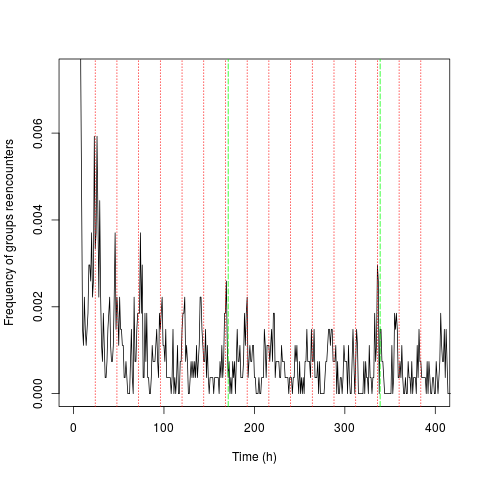
\includegraphics[width=1.7in]{group_reencounters.png}\label{peri_mit}}
  \subfigure[Dartmouth (Real Trace)]{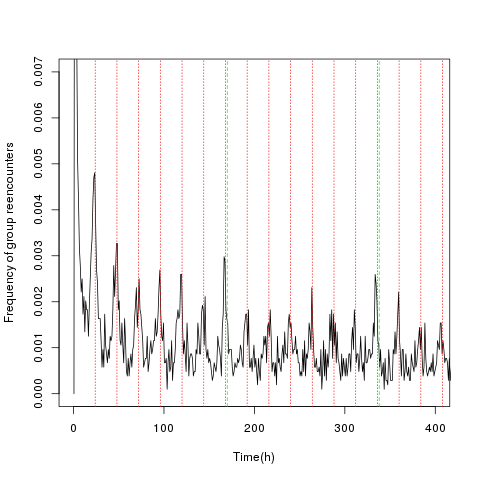
\includegraphics[width=1.7in]{dart_periodicity.png}\label{peri_dartmouth}}
  \subfigure[SWIM (Synthetic Trace)]{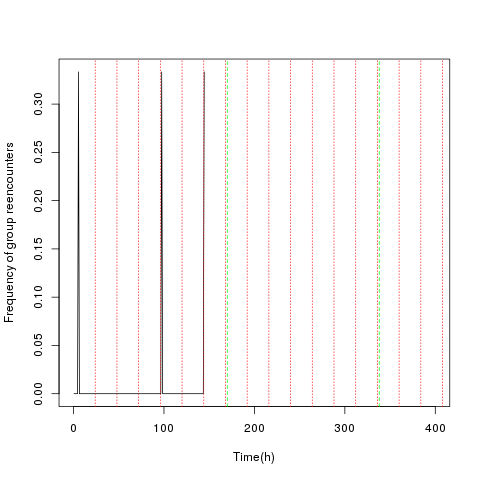
\includegraphics[width=1.7in]{swim_periodicity.png}\label{peri_swim}}
  \subfigure[WDM (Synthetic Trace)]{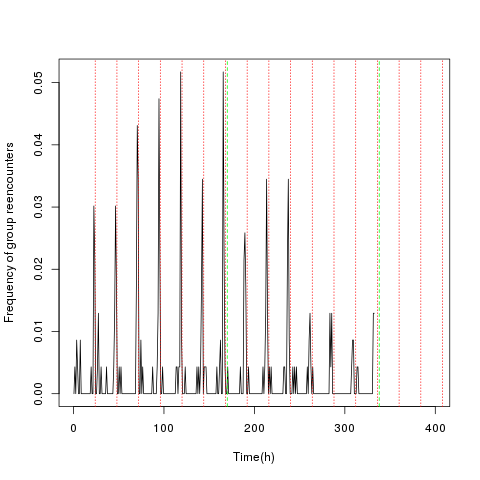
\includegraphics[width=1.7in]{wdm_periodicity.png}\label{peri_wdm}}
\caption{Comparison of group meetings periodicity in real and synthetic mobility traces}\label{periodicity}
\end{figure}

In this section we compare some of the state-of-art and widely used synthetic mobility models with real mobility traces, with the goal of verifying if group meetings' regularity properties are captured by such synthetic models. Specifically, we want to see if such models capture group re-encounters and their evolution over time to be able to decide if they are representative, considering the group mobility feature and if they should or not be used in the validation of opportunistic networking protocols based on group meetings and social context.

Firstly, we apply the methodology for detecting and tracking groups, proposed by Nunes et al. \cite{icc} to both real mobility traces, MIT and Dartmouth. Figures~\ref{peri_mit} and \ref{peri_dartmouth} show the P.D.F. of group re-meetings along the time for the real world traces. In both of the real mobility traces we can verify the presence of periodicity in groups' re-encounters. By looking at both of them, we see that the mass of probability is concentrated in peaks aroud the red dotted lines, which represent periods of 24 hours. We also observe in both figures~\ref{peri_mit} and \ref{peri_dartmouth} that higher peaks are presented around the green dashed lines, which represent periods of seven days. This pattern in the group re-meetings' P.D.F. shows that group meetings present daily and weekly periodicity. It is noteworthy that such pattern is observed in both of the real traces, even though they are from different places, have different number of nodes, and used different data collection methods. Next, we leverage three widely used state-of-art synthetic mobility models to verify if they represent well the role of social groups to mobility.

The SWIM mobility model was introduced by Mei and Stefa \cite{swim} as a model to generate synthetic small worlds which preserve the pairwise contact duration and inter-contact times statistical distributions as they are observed in real mobility traces. The SLAW mobility model \cite{slaw} was designed to capture several significant statistical patterns of human mobility, including truncated power-law distributions of human displacements, pause-times and pairwise inter-contact times, fractal way-points, and heterogeneously defined areas of individual mobility. The Working Day Movement (WDM) synthetic model \cite{wdm} is a model designed to capture these same statical properties of contact durations and inter-contact times as SWIM and SLAW. In addition to those properties, WDM aims to capture the daily regularity of human movements, i.e., how human routines after their mobility.

As we did for the real traces, MIT and Dartmouth, we have applied the same group detection and tracking methodology to the contact traces generated by these three synthetic models. Figures \ref{peri_swim} and \ref{peri_wdm} present the results for the SWIM and WDM models, respectively.

The contact trace generated by the SWIM model (figure \ref{peri_swim}) do not present any regularity in group meetings. Out of the detected groups only three group re-meetings were registered in a period of 15 days. The result for the contact trace generated by the SLAW model presented an analogous behavior, i.e., no regularity in group meetings. This behavior is explained by the fact that such models were designed to be representative of the statistical properties of pairwise contacts only, without considering that human contacts often involve more than two peers. These models look only at pairwise contacts, disregarding group meetings.

In the WDM trace (figure \ref{peri_wdm}) we can observe that group re-meetings happen precisely in periods of 24 hours and with much higher frequencies than in real mobility traces. This behavior is observed because WDM firstly defines a set of places, called offices, and than distribute nodes to transition between pre-defined subsets of offices with daily periodicity. Therefore, nodes with intersections in their lists of offices will always form groups with exaggerated meeting regularity.

By analysing the group meetings regularity of the synthetic models, we conclude that none of them represent well the group mobility patterns. For this reason, none of the synthetic models fit for evaluating social-aware opportunistic routing strategies. Therefore, in section \ref{sec:model}, we propose GRM, a group dynamics aware mobility model which comprise the statistical properties of group meetings regularity.

\section{GRM Model}\label{sec:model}



\subsection{The intuition}



\begin{figure}[!t]
\centering
\includegraphics[width=2.2in]{GDM.png}
\caption{GDM Model Framework}\label{GDM}
\end{figure}

\subsection{Group Meeting Times}

% To properly design a mobility model for group dynamics, there must be a representative statistical model for group meetings regularity. Due to group meetings' periodicity, presented in Figure \ref{periodicity}, it makes sense to model such behavior as a Poisson process. In a Poisson process, the accumulated number of occurrences along the time must be well approximated by a straight line with slope $\lambda$. To verify the goodness of fit of group meetings to a Poisson process, for each group in the trace, we perform a linear regression of the number of meetings over time. Then, we compute the $R^2$ value of each group, which measures how well the linear model fits to the number of meetings. Figure \ref{poisson} exemplifies such regression for different values of $R^2$. Figure \ref{R2}, which presents the frequency distribution of $R^2$ for all groups in the trace, shows that group meetings have a good fit to a Poisson process, most of them with $R^2$ values of 0.85 or higher. We use this Poisson process model to design our model. 

% We start designing our model based on the observation that group meetings' times can be well approximated by a Poisson process. Following this assumption, the probability of a given group to meet $K$ times in the $t$-time interval is given by the expression:

% \begin{equation}
% P[N(t) = K] = \frac{e^{-\lambda t}(\lambda t)^K}{K!}.
% \end{equation}

% Therefore, the probability $F(t)$ of a group re-meeting until a given time $t$ is:

% \begin{equation}\label{eq3}
% F(t) = P[N(t) \geqslant 1] = 1 - P[N(t) = 0] = 1 - e^{-\lambda t}.
% \end{equation}

% Basically, Eq.~\ref{eq3} shows that the more time passes, the more likely it is that a group re-meeting will occur. Next, we find the inverse function of $F(t)$ (Eq.~\ref{eq3}):

% We are able to use an uniformly distributed random variable, namely $U$, assuming values in the interval $[0,1] \in \mathbb{R}$, to generate group meetings times according to a Poisson process.

% \begin{equation}\label{eq4}
% \begin{split}
% F(t) = 1 - e^{-\lambda t} \implies\\
% e^{-\lambda t} = 1 - F(t) \implies\\
% \lambda t = -ln(1-F(t)) \implies\\
% t = \frac{-ln(1-F(t))}{\lambda}
% \end{split}
% \end{equation}

% By using the inverse function of $F(t)$, we are able to use an uniformly distributed random variable, namely $U$, assuming values in the interval $[0,1] \in \mathbb{R}$, to generate group meeting times that follow a Poisson process:

% \begin{equation}\label{eq5}
% NextMeetingTime = \frac{-ln(U)}{\lambda}
% \end{equation}

% Eq. \ref{eq5} provides a systematic way for generating periodic re-meeting times for a given group. It relies on the $\lambda$ parameter to define if a group will be more or less frequent.
% Intuitively, different groups should have different inter-meeting times. Thus, different groups should have different values of $\lambda$. To generate representative synthetic data we evaluate the $\lambda$ values frequencies for groups detected in real world traces.  

% \begin{equation}\label{eq6}
% \lambda(\mu,\sigma) = N(\mu,\sigma)
% \end{equation}

% However, in reality, group meetings do no perfectly follow a a Poisson process, thus we add to hour model a white normal noise, i.e., we sum a random error with normal distribution to each of the meeting times generated by the Poisson Point Process. 

% \begin{figure}[!t]
% \centering
%   \subfigure[]{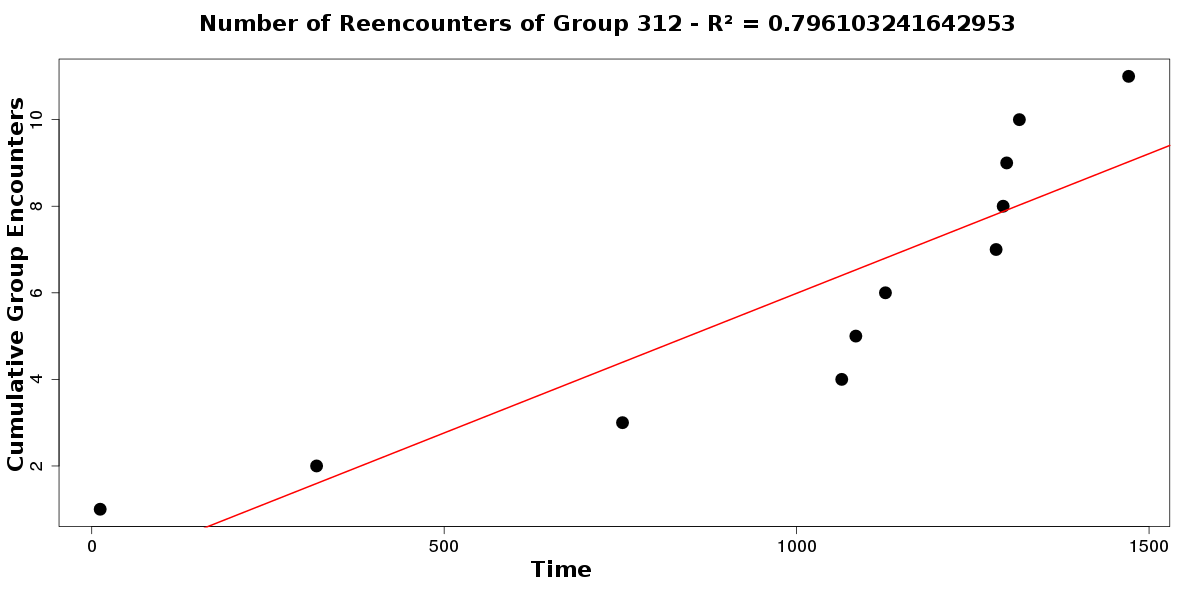
\includegraphics[width=1.7in]{poisson1.png}\label{p1}}
%   \subfigure[]{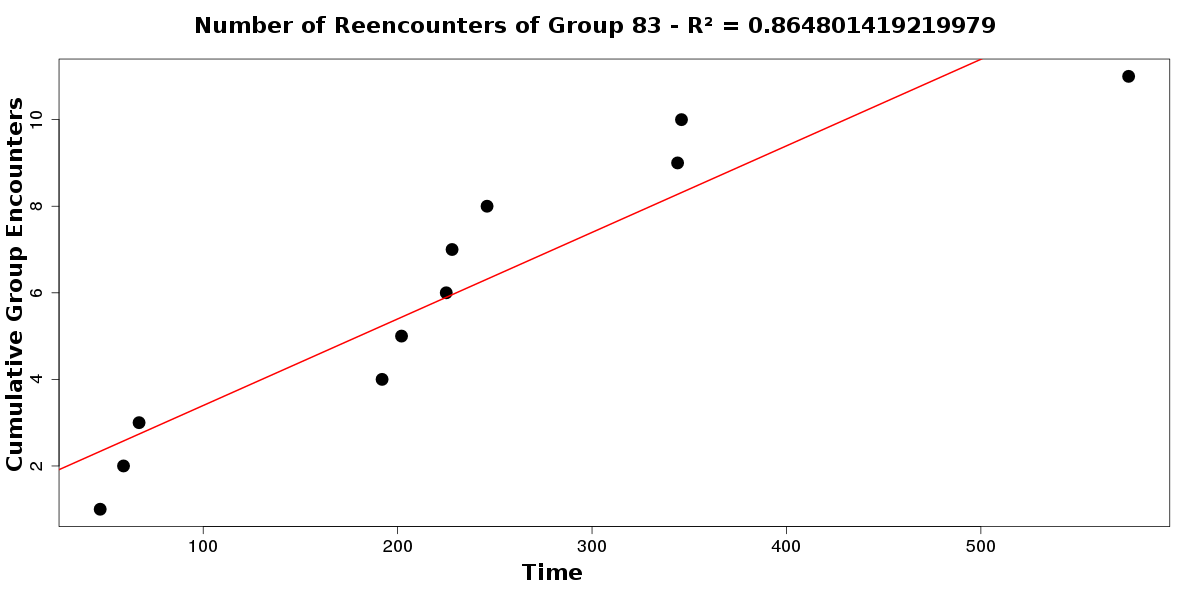
\includegraphics[width=1.7in]{poisson2.png}\label{p2}}
%   \subfigure[]{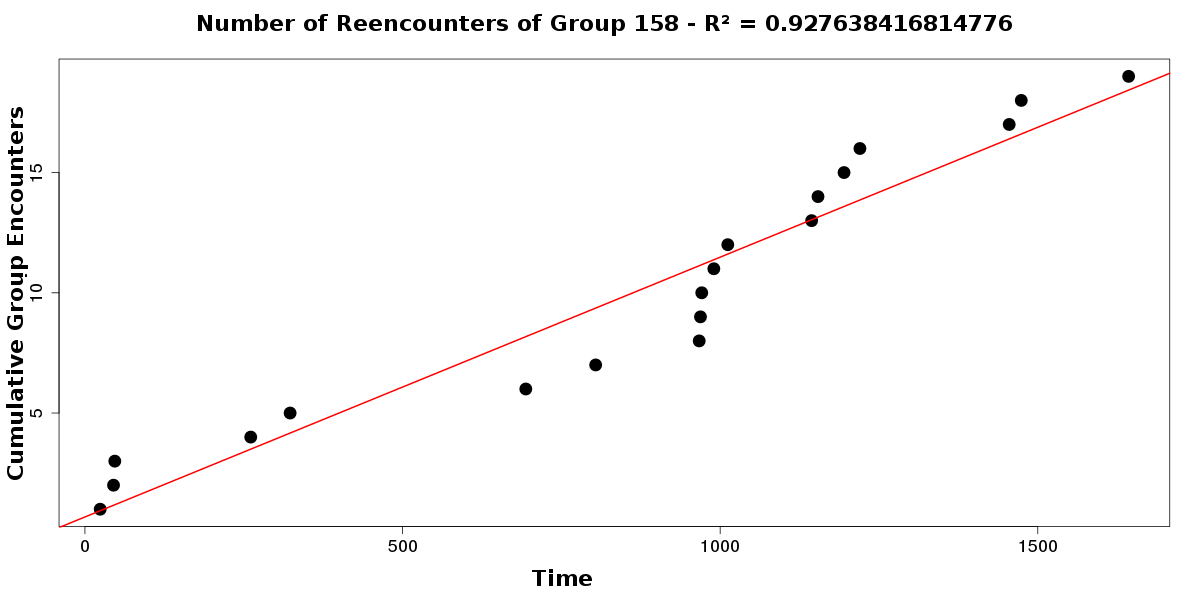
\includegraphics[width=1.7in]{poisson3.png}\label{p3}}
%   \subfigure[]{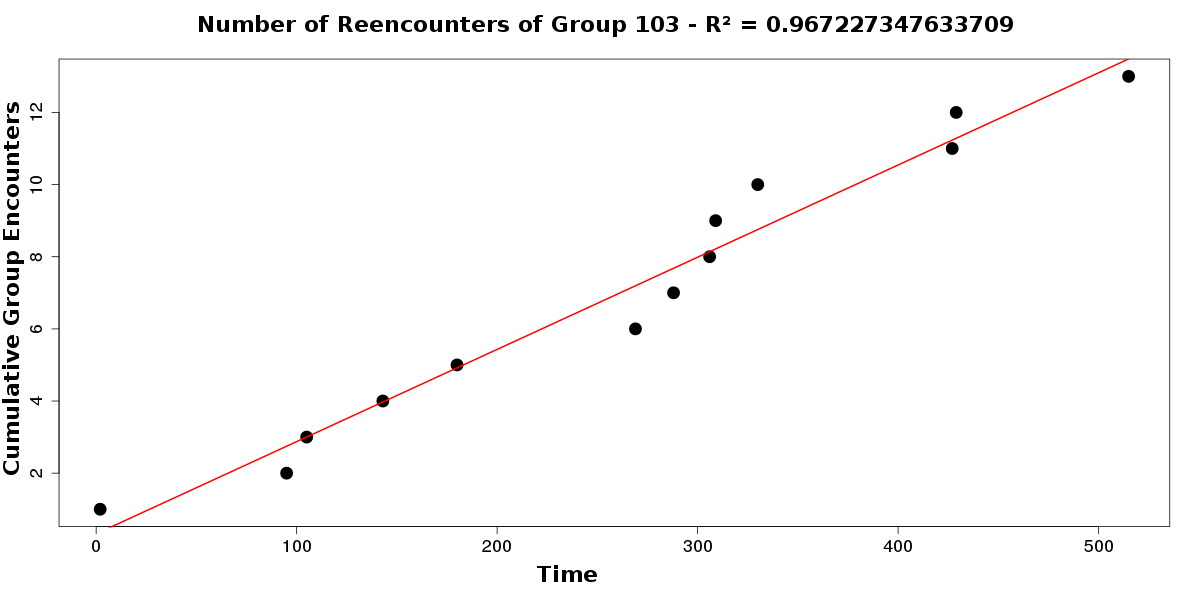
\includegraphics[width=1.7in]{poisson4.png}\label{p4}}
% \caption{Poisson process fit for different values of $R^2$}\label{poisson}
% \end{figure}

% \begin{figure}[!t]
% \centering
% 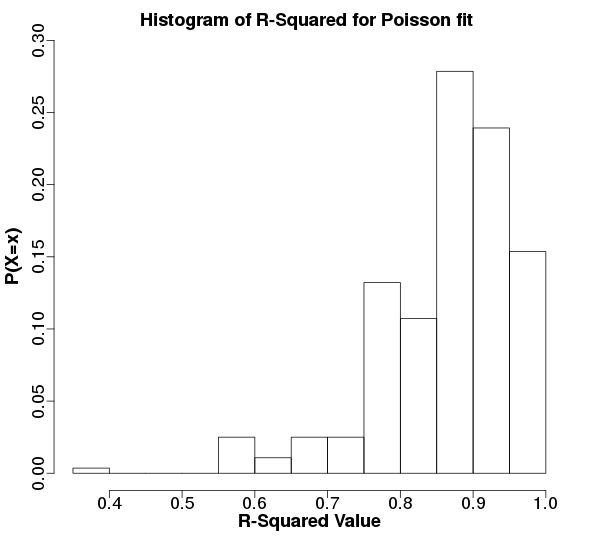
\includegraphics[width=2.2in]{poisson5.png}
% \caption{R-squared distribution for Poisson distribution fits of each group of the trace}\label{R2}
% \end{figure}


% \begin{figure}[!t]
% \centering
%   \subfigure[Pure Poisson process]{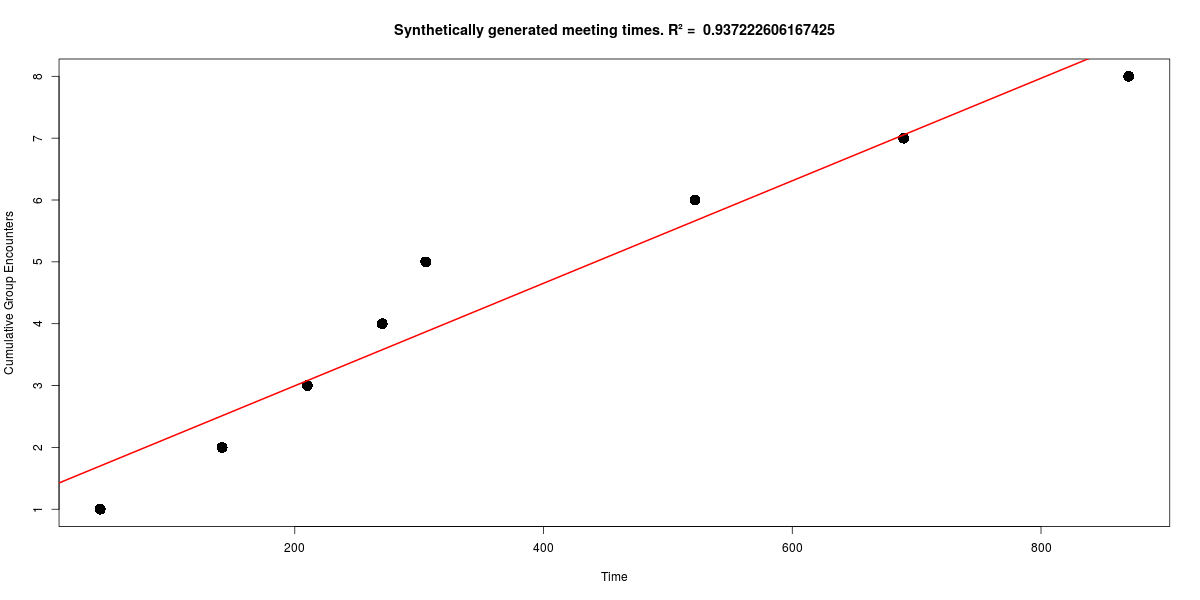
\includegraphics[width=1.7in]{synth_poisson.png}\label{pure}}
%   \subfigure[Poisson process plus Normal Noise]{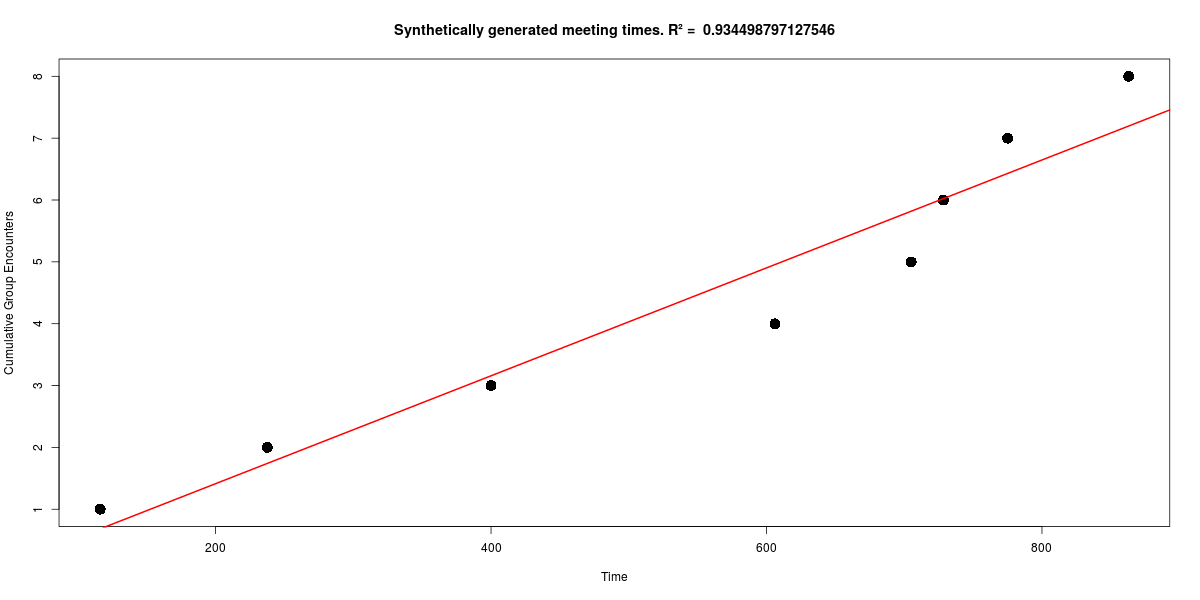
\includegraphics[width=1.7in]{noise.png}\label{noise}}
% \caption{}\label{synth_poisson}
% \end{figure}

\begin{figure}[!t]
\centering
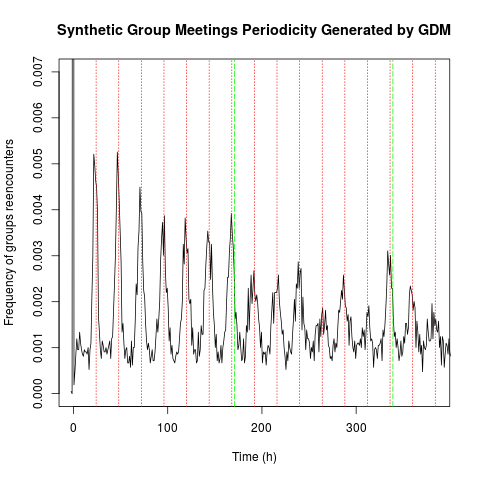
\includegraphics[width=\columnwidth]{best_periodicity.png}
\caption{GRM Model Group Re-Meetings}\label{GRM}
\end{figure}

\subsection{Group Sizes}

Generate according to a probability distribution function according to the MIT and Dartmouth characterization;

\begin{itemize}
    \item rexp?
    \item rnorm?
    \item The parameters (e.g., $\mu, \sigma$ ) are simulation parameters. Each of the $\#g$ groups ($\#g$ is a simulation parameter) are attributed with a group size;
\end{itemize}

\begin{figure}[!t]
\centering
  \subfigure[Average group size of 6.06]{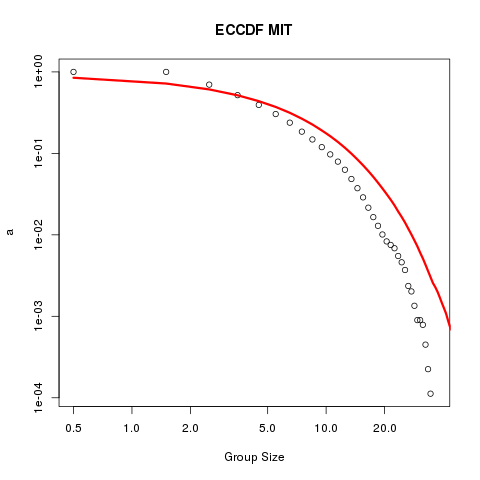
\includegraphics[width=1.7in]{mit_group_size.png}\label{mit_g_size}}
  \subfigure[Average group size of 6.96]{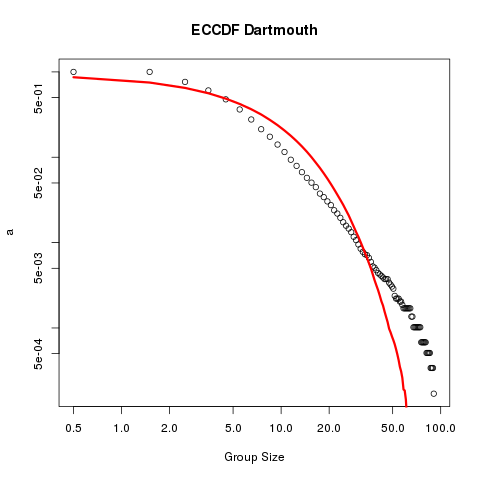
\includegraphics[width=1.7in]{dart_group_size.png}\label{dt_g_size}}
\caption{Group sizes}\label{comm}
\end{figure}

\subsection{Group Members and Social Context}

\begin{figure}[!t]
\centering
  \subfigure[Dartmouth (Real Trace)]{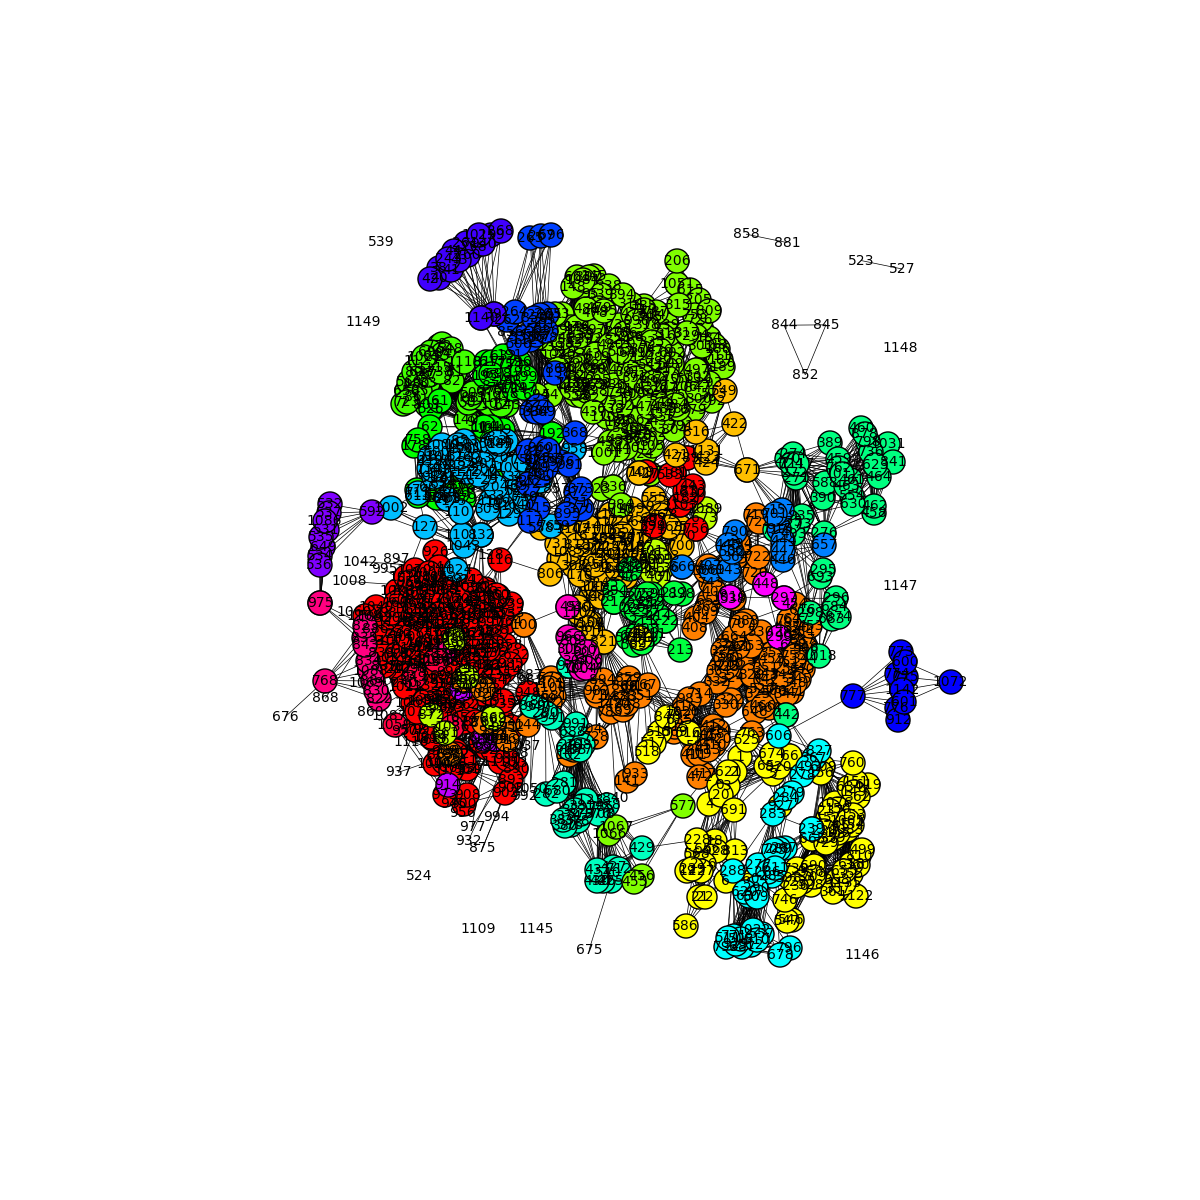
\includegraphics[width=1.7in]{dartmouth.png}\label{dartmouth_net}}
  \subfigure[Barabasi-Albert (Synthetic Network Model)]{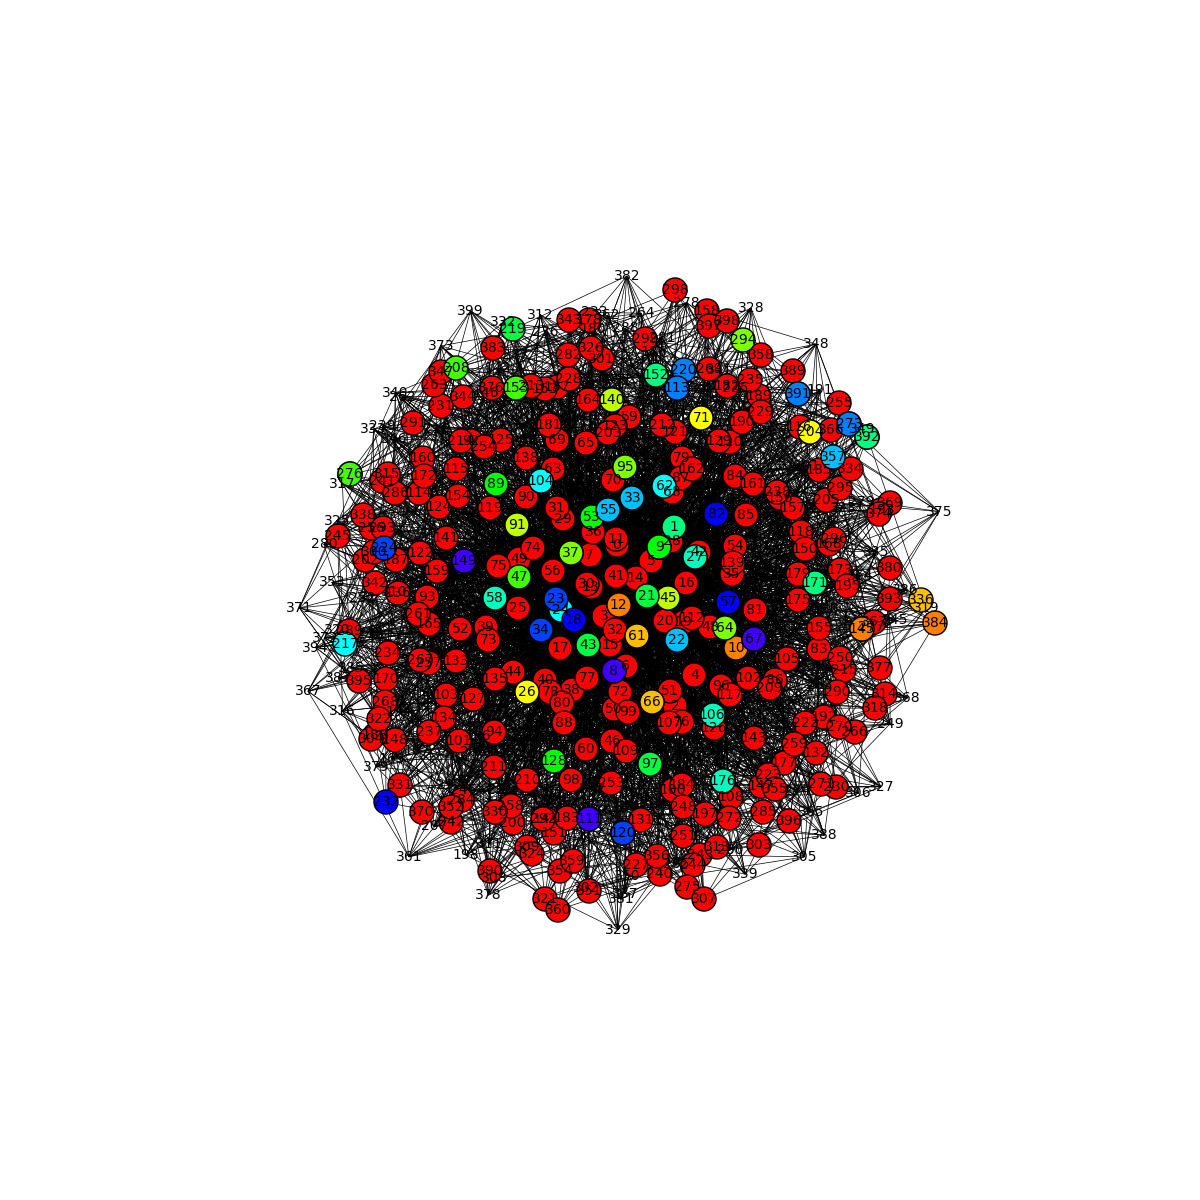
\includegraphics[width=1.7in]{barabasi.png}\label{barabasi_net}}
  \subfigure[Ex1 of Gaussian Clustering Model (Synthetic Network Model)]{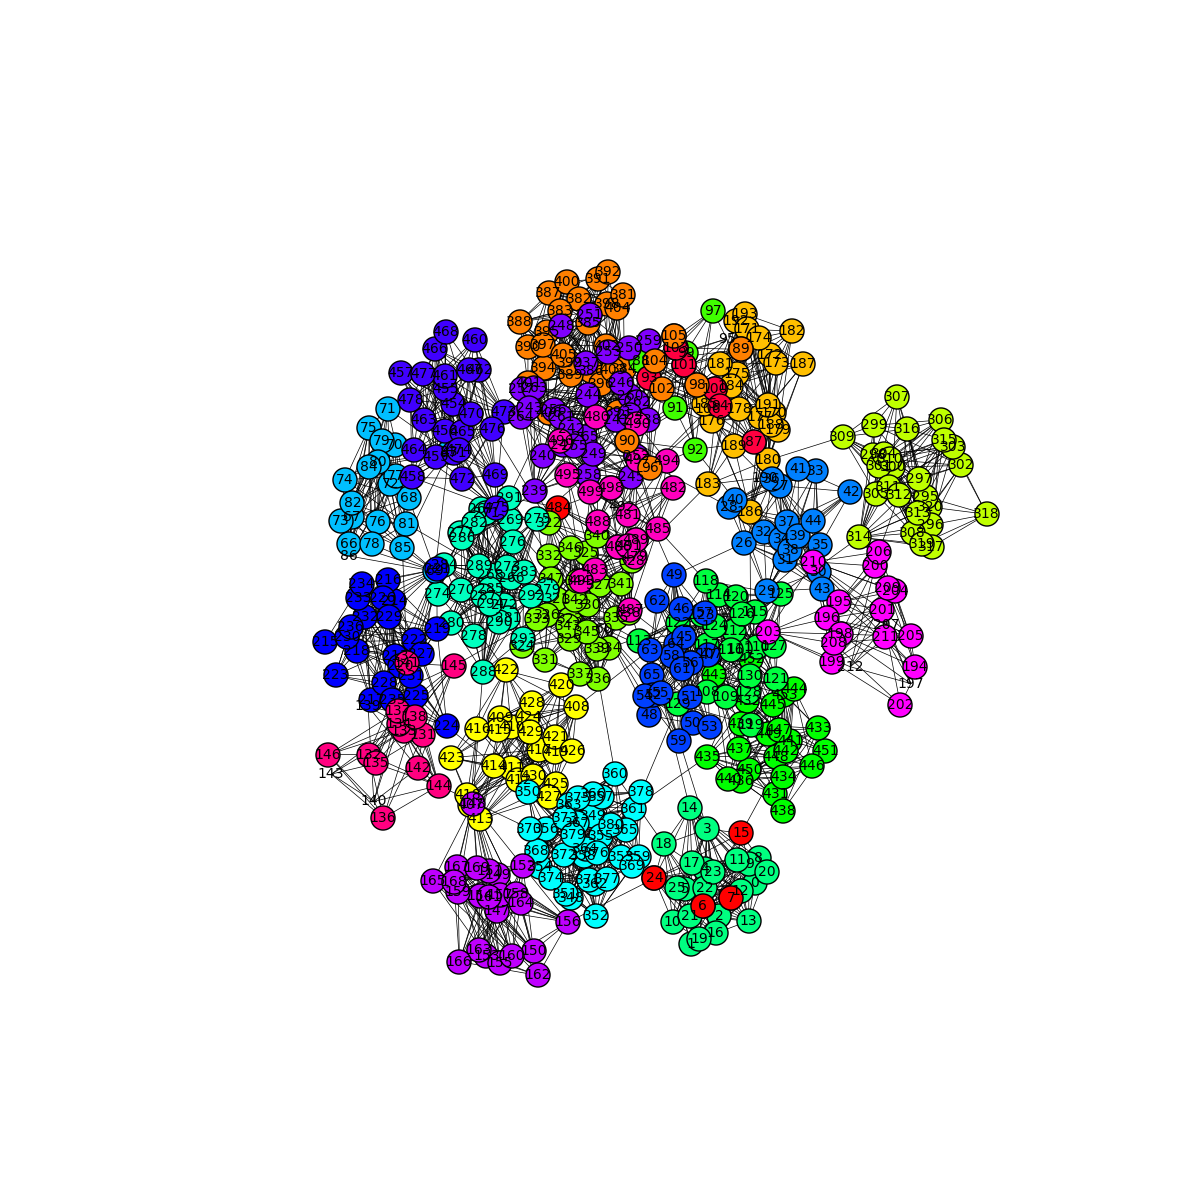
\includegraphics[width=1.7in]{gaussian.png}\label{gaussian_net1}}
  \subfigure[Ex2 of Gaussian Clustering Model (Synthetic Network Model)]{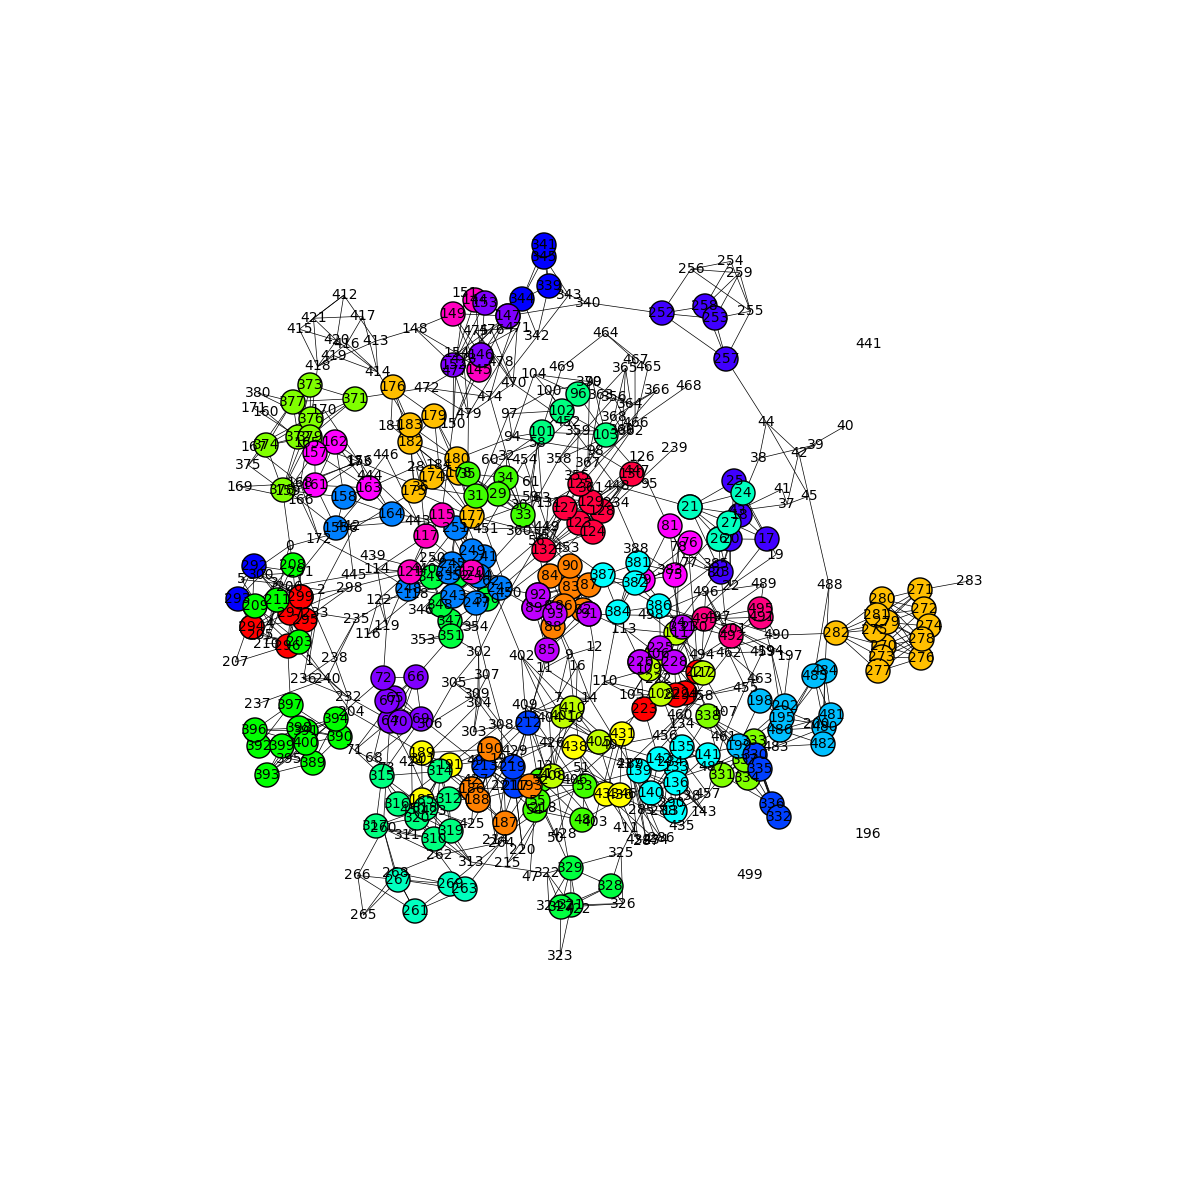
\includegraphics[width=1.7in]{gaussian2.png}\label{gaussian_net2}}
\caption{Comparison of community structures}\label{comm}
\end{figure}

Select $\#g$ group leaders with uniform distribution in the set of users in the traces $[0, n] \in N$, where $n$ is the number of nodes to be simulated and $\#g$ the number of groups. Both $\#g$ and $n$ are given as parameters to the model.

Each group leader then invites the number of members of its group using a Snowball algorithm. The Snowball algorithm, firstly assembles a social-contact graph and selects the node with the highest centrality. Next, it adds to the subset of nodes the neighbors of the central node. Then, it adds the neighbors of such neighbors and so on, until the desired number of nodes for the subset is reached. This way, the social structure of the network is preserved:

Let $G_i$ be the set of nodes that compose the group $i \in [0,n]$

\begin{equation}\label{eq7}
\begin{split}
G_i.size = N(\mu,\sigma)\\
G_i.nodes = Snowball(Leader_i,G_i.size,SocialGraph)
\end{split}
\end{equation}

To each user $j$ in $G_i.nodes$, a probability of attending to a $G_i$ meeting is assigned as follows:

\begin{equation}\label{eq8}
\begin{split}
P_{attendance}[User_j]= \frac{\#KnownGuests(User_j,G_i.nodes)}{G_i.size}
\end{split}
\end{equation}

For each of the $G_i$ meetings, each of the users $j$ in $G_i.nodes$ participate with probability $P_{attendance}[User_j]$.

\subsection{Group Meetings Durations}

\subsubsection{Early Leaving and Late Arrival}



\subsection{Implementation and Usage}



\section{GRM vs Real Mobility}

\begin{itemize}
    \item Group meetings regularity.
    \item Community structure
    \item Inter-contact times
    \item Contact Duration
\end{itemize}


\section{Opportunistic Networking in GRM Synthetic Traces}



\section{Conclusion}\label{conclusion}



\section*{Acknowledgment}

\ifCLASSOPTIONcaptionsoff
  \newpage
\fi

\bibliographystyle{IEEEtran}
\bibliography{main}

\begin{IEEEbiography}[{\includegraphics[width=1in,height=1.25in,clip,keepaspectratio]{picture}}]{John Doe}

\end{IEEEbiography}


\end{document}
